\documentclass[tikz,border=12pt]{standalone}
\usepackage[T1]{fontenc}
\usepackage{lmodern,amsmath,amssymb}
\usetikzlibrary{arrows.meta,positioning}
\definecolor{ink}{HTML}{183444}
\definecolor{blue}{HTML}{1B6780}
\definecolor{amber}{HTML}{AD601A}
\begin{document}
\hyphenpenalty=10000\exhyphenpenalty=10000
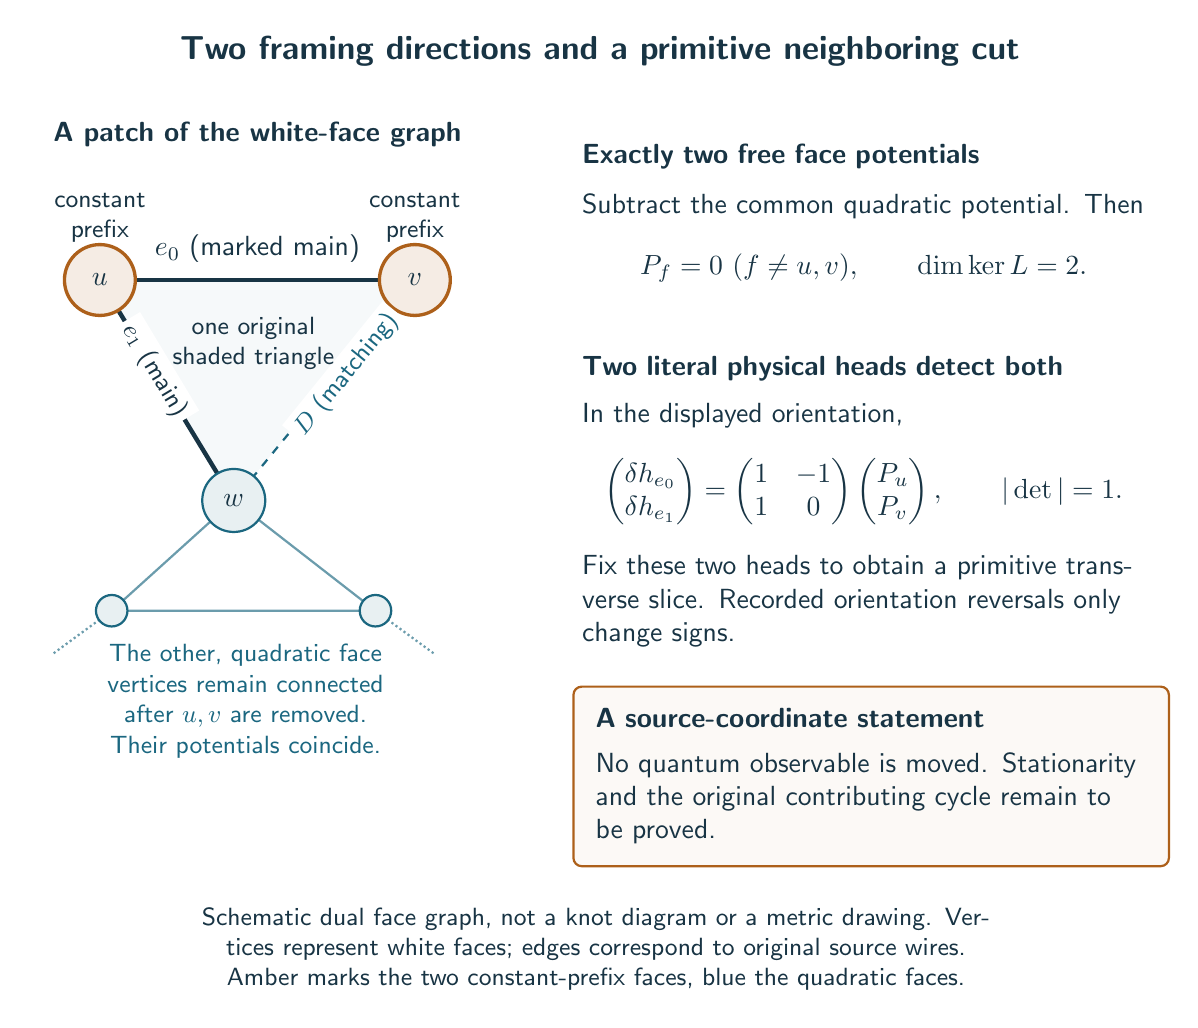
\begin{tikzpicture}[font=\sffamily,text=ink,>=Stealth,
 constant/.style={circle,draw=amber,fill=amber!12,very thick,
                  minimum size=9mm,inner sep=1pt},
 quadratic/.style={circle,draw=blue,fill=blue!10,thick,
                   minimum size=8mm,inner sep=1pt}]

 \node[font=\sffamily\large\bfseries] at (6.35,3.6)
 {Two framing directions and a primitive neighboring cut};

 \node[font=\sffamily\bfseries,align=center] at (2,2.55)
 {A patch of the white-face graph};
 \coordinate (U) at (0,.7);
 \coordinate (V) at (4,.7);
 \coordinate (W) at (1.7,-2.1);
 \coordinate (X) at (.15,-3.5);
 \coordinate (Y) at (3.5,-3.5);

 \fill[blue!4] (U)--(V)--(W)--cycle;
 \draw[ink,line width=1.6pt] (U)--(V);
 \draw[ink,line width=1.6pt] (U)--(W);
 \draw[blue,thick,dashed] (V)--(W);
 \draw[blue!65,thick] (W)--(X)--(Y)--(W);
 \draw[blue!65,densely dotted,thick] (X)--(-.6,-4.05);
 \draw[blue!65,densely dotted,thick] (Y)--(4.25,-4.05);

 \node[constant] at (U) {$u$};
 \node[constant] at (V) {$v$};
 \node[quadratic] at (W) {$w$};
 \node[quadratic,minimum size=4mm] at (X) {};
 \node[quadratic,minimum size=4mm] at (Y) {};

 \node[above=10pt,font=\sffamily\small,align=center] at (U)
 {constant\\prefix};
 \node[above=10pt,font=\sffamily\small,align=center] at (V)
 {constant\\prefix};
 \node[above=4pt,fill=white,inner sep=2pt] at (2,.7)
 {$e_0$ (marked main)};
 \node[rotate=-59,fill=white,inner sep=2pt,font=\sffamily\small]
 at (.69,-.45) {$e_1$ (main)};
 \node[rotate=51,fill=white,inner sep=2pt,font=\sffamily\small,text=blue]
 at (3.13,-.5) {$D$ (matching)};
 \node[align=center,font=\sffamily\small] at (1.95,-.1)
 {one original\\shaded triangle};
 \node[blue,align=center,font=\sffamily\small,text width=5.3cm]
 at (1.85,-4.65)
 {The other, quadratic face vertices remain connected\\
 after $u,v$ are removed. Their potentials coincide.};

 \node[anchor=north west,align=left,text width=7.15cm]
 at (6,2.55) {
  \textbf{Exactly two free face potentials}\\[6pt]
  Subtract the common quadratic potential. Then
  \[P_f=0\ (f\ne u,v),\qquad \dim\ker L=2.\]};

 \node[anchor=north west,align=left,text width=7.15cm]
 at (6,-.15) {
  \textbf{Two literal physical heads detect both}\\[5pt]
  In the displayed orientation,
  \[
  \begin{pmatrix}\delta h_{e_0}\\ \delta h_{e_1}\end{pmatrix}
  =\begin{pmatrix}1&-1\\1&0\end{pmatrix}
   \begin{pmatrix}P_u\\P_v\end{pmatrix},
  \qquad |\det|=1.
  \]
  Fix these two heads to obtain a primitive transverse slice.
  Recorded orientation reversals only change signs.};

 \node[draw=amber,thick,rounded corners=3pt,fill=amber!4,
       align=left,text width=7cm,inner sep=8pt,anchor=north west]
 at (6,-4.45) {
  \textbf{A source-coordinate statement}\\[4pt]
  No quantum observable is moved. Stationarity and the original
  contributing cycle remain to be proved.};

 \node[font=\sffamily\small,align=center,text width=13.6cm]
 at (6.3,-7.8) {
  Schematic dual face graph, not a knot diagram or a metric drawing.
  Vertices represent white faces; edges correspond to original source wires.
  Amber marks the two constant-prefix faces, blue the quadratic faces.};
\end{tikzpicture}
\end{document}
